\documentclass[12pt]{report}
\usepackage[utf8]{inputenc}
\usepackage[russian]{babel}
%\usepackage[14pt]{extsizes}
\usepackage{listings}
\usepackage{graphicx}
\usepackage{amsmath,amsfonts,amssymb,amsthm,mathtools} 
\usepackage{pgfplots}
\usepackage{filecontents}
\usepackage{float}
\usepackage{comment}
\usepackage{indentfirst}
\usepackage{eucal}
\usepackage{enumitem}
%s\documentclass[openany]{book}
\frenchspacing

\usepackage{array}

\usepackage{verbatim}

\usepackage{caption}
\captionsetup{labelsep=endash}
\captionsetup[figure]{name={Рисунок}}

\usepackage{indentfirst} % Красная строка

\usetikzlibrary{datavisualization}
\usetikzlibrary{datavisualization.formats.functions}

\usepackage{amsmath}


% Для листинга кода:
\lstset{ %
	language=c,                 % выбор языка для подсветки (здесь это С)
	basicstyle=\small\sffamily, % размер и начертание шрифта для подсветки кода
	numbers=left,               % где поставить нумерацию строк (слева\справа)
	numberstyle=\tiny,           % размер шрифта для номеров строк
	stepnumber=1,                   % размер шага между двумя номерами строк
	numbersep=5pt,                % как далеко отстоят номера строк от подсвечиваемого кода
	showspaces=false,            % показывать или нет пробелы специальными отступами
	showstringspaces=false,      % показывать или нет пробелы в строках
	showtabs=false,             % показывать или нет табуляцию в строках
	frame=single,              % рисовать рамку вокруг кода
	tabsize=2,                 % размер табуляции по умолчанию равен 2 пробелам
	captionpos=t,              % позиция заголовка вверху [t] или внизу [b] 
	breaklines=true,           % автоматически переносить строки (да\нет)
	breakatwhitespace=false, % переносить строки только если есть пробел
	escapeinside={\#*}{*)}   % если нужно добавить комментарии в коде
}


\usepackage[left=2cm,right=2cm, top=2cm,bottom=2cm,bindingoffset=0cm]{geometry}
% Для измененных титулов глав:
\usepackage{titlesec, blindtext, color} % подключаем нужные пакеты
\definecolor{gray75}{gray}{0.75} % определяем цвет
\newcommand{\hsp}{\hspace{20pt}} % длина линии в 20pt
% titleformat определяет стиль
\titleformat{\chapter}[hang]{\Huge\bfseries}{\thechapter\hsp\textcolor{gray75}{|}\hsp}{0pt}{\Huge\bfseries}


% plot
\usepackage{pgfplots}
\usepackage{filecontents}
\usetikzlibrary{datavisualization}
\usetikzlibrary{datavisualization.formats.functions}

\begin{document}
	%\def\chaptername{} % убирает "Глава"
	\thispagestyle{empty}
	\begin{titlepage}
		\noindent \begin{minipage}{0.15\textwidth}
			
\includegraphics[width=\linewidth]{inc/b_logo}
		\end{minipage}
		\noindent\begin{minipage}{0.9\textwidth}\centering
			\textbf{Министерство науки и высшего образования Российской Федерации}\\
			\textbf{Федеральное государственное бюджетное образовательное учреждение высшего образования}\\
			\textbf{~~~«Московский государственный технический университет имени Н.Э.~Баумана}\\
			\textbf{(национальный исследовательский университет)»}\\
			\textbf{(МГТУ им. Н.Э.~Баумана)}
		\end{minipage}
		
		\noindent\rule{18cm}{3pt}
		\newline\newline
		\noindent ФАКУЛЬТЕТ $\underline{\text{«Информатика и системы управления»}}$ \newline\newline
		\noindent КАФЕДРА $\underline{\text{«Программное обеспечение ЭВМ и информационные технологии»}}$\newline\newline\newline\newline\newline
		
		\begin{center}
			\noindent\begin{minipage}{1.1\textwidth}\centering
				\Large\textbf{Отчет по лабораторной работе №1}\newline
				\textbf{по дисциплине <<Моделирование>>}\newline\newline
			\end{minipage}
		\end{center}
		
		\noindent\textbf{Тема} $\underline{\text{Распределение случайных величин}}$\newline\newline
		\noindent\textbf{Студент} $\underline{\text{Слепокурова М.Ф.}}$\newline\newline
		\noindent\textbf{Группа} $\underline{\text{ИУ7-76Б}}$\newline\newline
		\noindent\textbf{Оценка (баллы)} $\underline{\text{~~~~~~~~~~~~~~~~~}}$\newline\newline
		\noindent\textbf{Преподаватель} $\underline{\text{Рудаков И.В.}}$\newline\newline\newline
		
		\begin{center}
			\vfill
			Москва~---~\the\year
			~г.
		\end{center}
	\end{titlepage}

\setcounter{page} {2}





\section*{Постановка задачи}
Реализовать программное обеспечение для построения графиков функции распределения и функции плотности вероятности для случайных чисел для равномерного распределения и распределения Эрланга.

\section*{Теория}
\subsection*{Равномерное распределение}
Равномерное распределение описывает случайную величину, принимающую значения, принадлежащие некоторому промежутку конечной длины, при этом плотность вероятности в этом промежутке всюду постоянна.
\newline

Функция распределения равномерной непрерывной случайной величины имеет следующий вид:
\begin{equation*}
	F(x) = \begin{cases}
		0, & x \leq a \\
		\frac{x-a}{b-a}, & a \leq x \leq b \\
		1, & x > b
	\end{cases}
\end{equation*}

Плотность распределения равномерной непрерывной случайной величины имеет следующий вид:
\begin{equation*}
	f(x) = \begin{cases}
		\frac{1}{b-a}, & a \leq x \leq b \\
		0, & \text{иначе}
	\end{cases}
\end{equation*}


\subsection*{Распределение Эрланга}
Распределение Эрланга описывает непрерывную случайную величину, принимающую неотрицательные значения и представляющую собой сумму $n$ независимых случайных величин, распределенных по одному и тому же экспоненциальному закону с параметром $\lambda$.
\newline

Функция распределения Эрланга непрерывной случайной величины имеет следующий вид:
\begin{equation*}
	F(x) = 1 - e^{-x/\lambda} \sum_{i=0}^{n-1} \frac{(x/\lambda)^i}{i!} 
\end{equation*}

Плотность распределения Эрланга непрерывной случайной величины имеет следующий вид:
\begin{equation*}
	f(x) = \frac{x^{n-1}e^{-x\lambda}\lambda^n}{(n-1)!}
\end{equation*}


\section*{Средства реализации}

Для реализации приложения был выбран язык программирования Python, в стандартную библиотеку которого входит графическая библиотека Tkinter, использовавшаяся для реализации пользовательского интерфейса.

\section*{Листинг кода}

\begin{lstlisting}
import math
import matplotlib
import numpy as np

def uniformDistribution(x, a, b):
  if a <= x < b:
    return (x - a) / (b - a)
  if x < a:
    return 0
  return 1

def uniformDistributionDensity(x, a, b):
  if a <= x <= b:
    return 1 / (b - a)
  return 0

def erlangDistribution(x, n, lmbd):
  return 1 - math.exp(-x / lmbd) * sum((x / lmbd)**i/math.factorial(i) for i in range(n))

def erlangDistributionDensity(x, n, lmbd):
  return x**(n - 1) * math.exp(-x * lmbd) * lmbd**n / math.factorial(n - 1)

def plotUniform(a, b, x1, x2):
  x = np.arange(x1, x2, 0.0001)
  y = [uniformDistribution(_x, a, b) for _x in x]
  y_density = [uniformDistributionDensity(_x, a, b) for _x in x]

  fig, axs = initCanvasFigure("Uniform distribution")
  drawCanvasFigure(axs, x, y, y_density)

  drawCanvasUniform(fig)

def plotErlang(n, lmbd, x1, x2):
  x = np.arange(x1, x2, 0.0001)
  y = [erlangDistribution(_x, n, lmbd) for _x in x]
  y_density = [erlangDistributionDensity(_x, n, lmbd) for _x in x]

  fig, axs = initCanvasFigure("Erlang distribution")
  drawCanvasFigure(axs, x, y, y_density)

  drawCanvasErlang(fig)
\end{lstlisting}


\section*{Демонстрация работы программы}
На рисунке \ref{fig:pic1} изображен пример работы программы для равномерного распределения с параметрами $a$ = -10, $b$ = 10 на отрезке [-20; 20] и для распределения Эрланга с параметрами $n$ = 1, $\lambda$ = 1 на отрезке [0; 10].

\begin{figure}[h!btp]
	\centering
	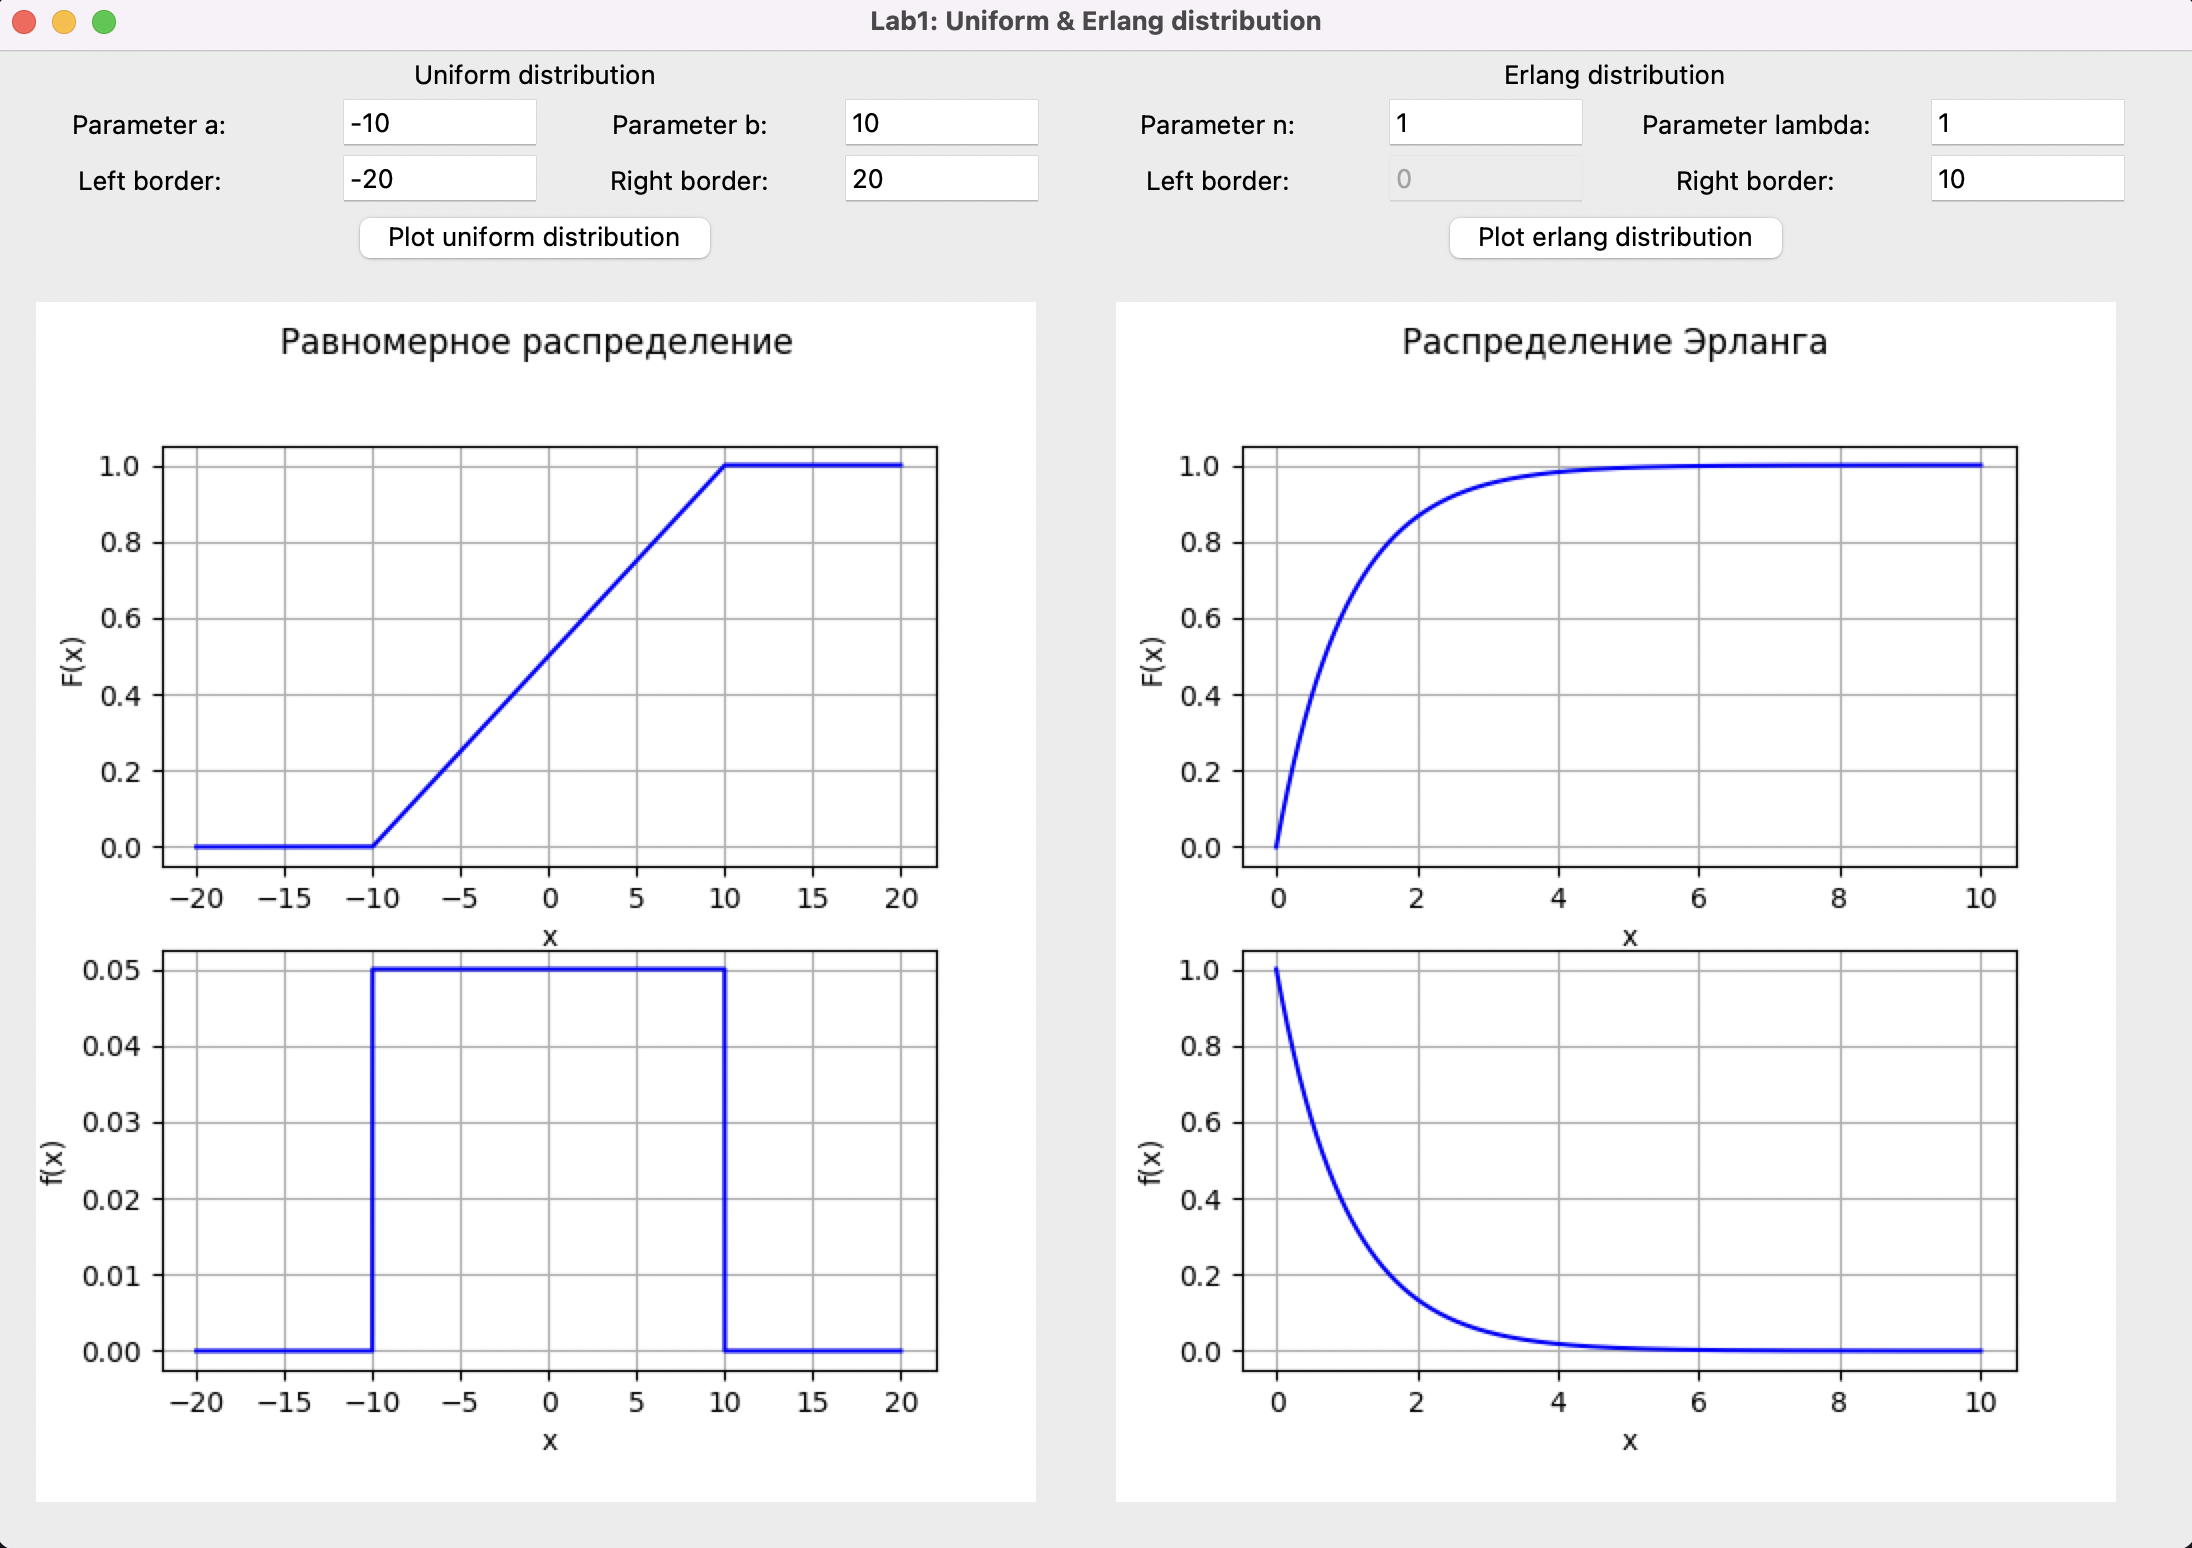
\includegraphics[width=1\textwidth]{inc/pic1.png}
	\caption{Пример работы программы --- 1}
	\label{fig:pic1}	
\end{figure}

\clearpage
На рисунке \ref{fig:pic2} изображен пример работы программы для равномерного распределения с параметрами $a$ = 5, $b$ = 15 на отрезке [0; 20] и для распределения Эрланга с параметрами $n$ = 10, $\lambda$ = 1 на отрезке [0; 20].

\begin{figure}[h!btp]
	\centering
	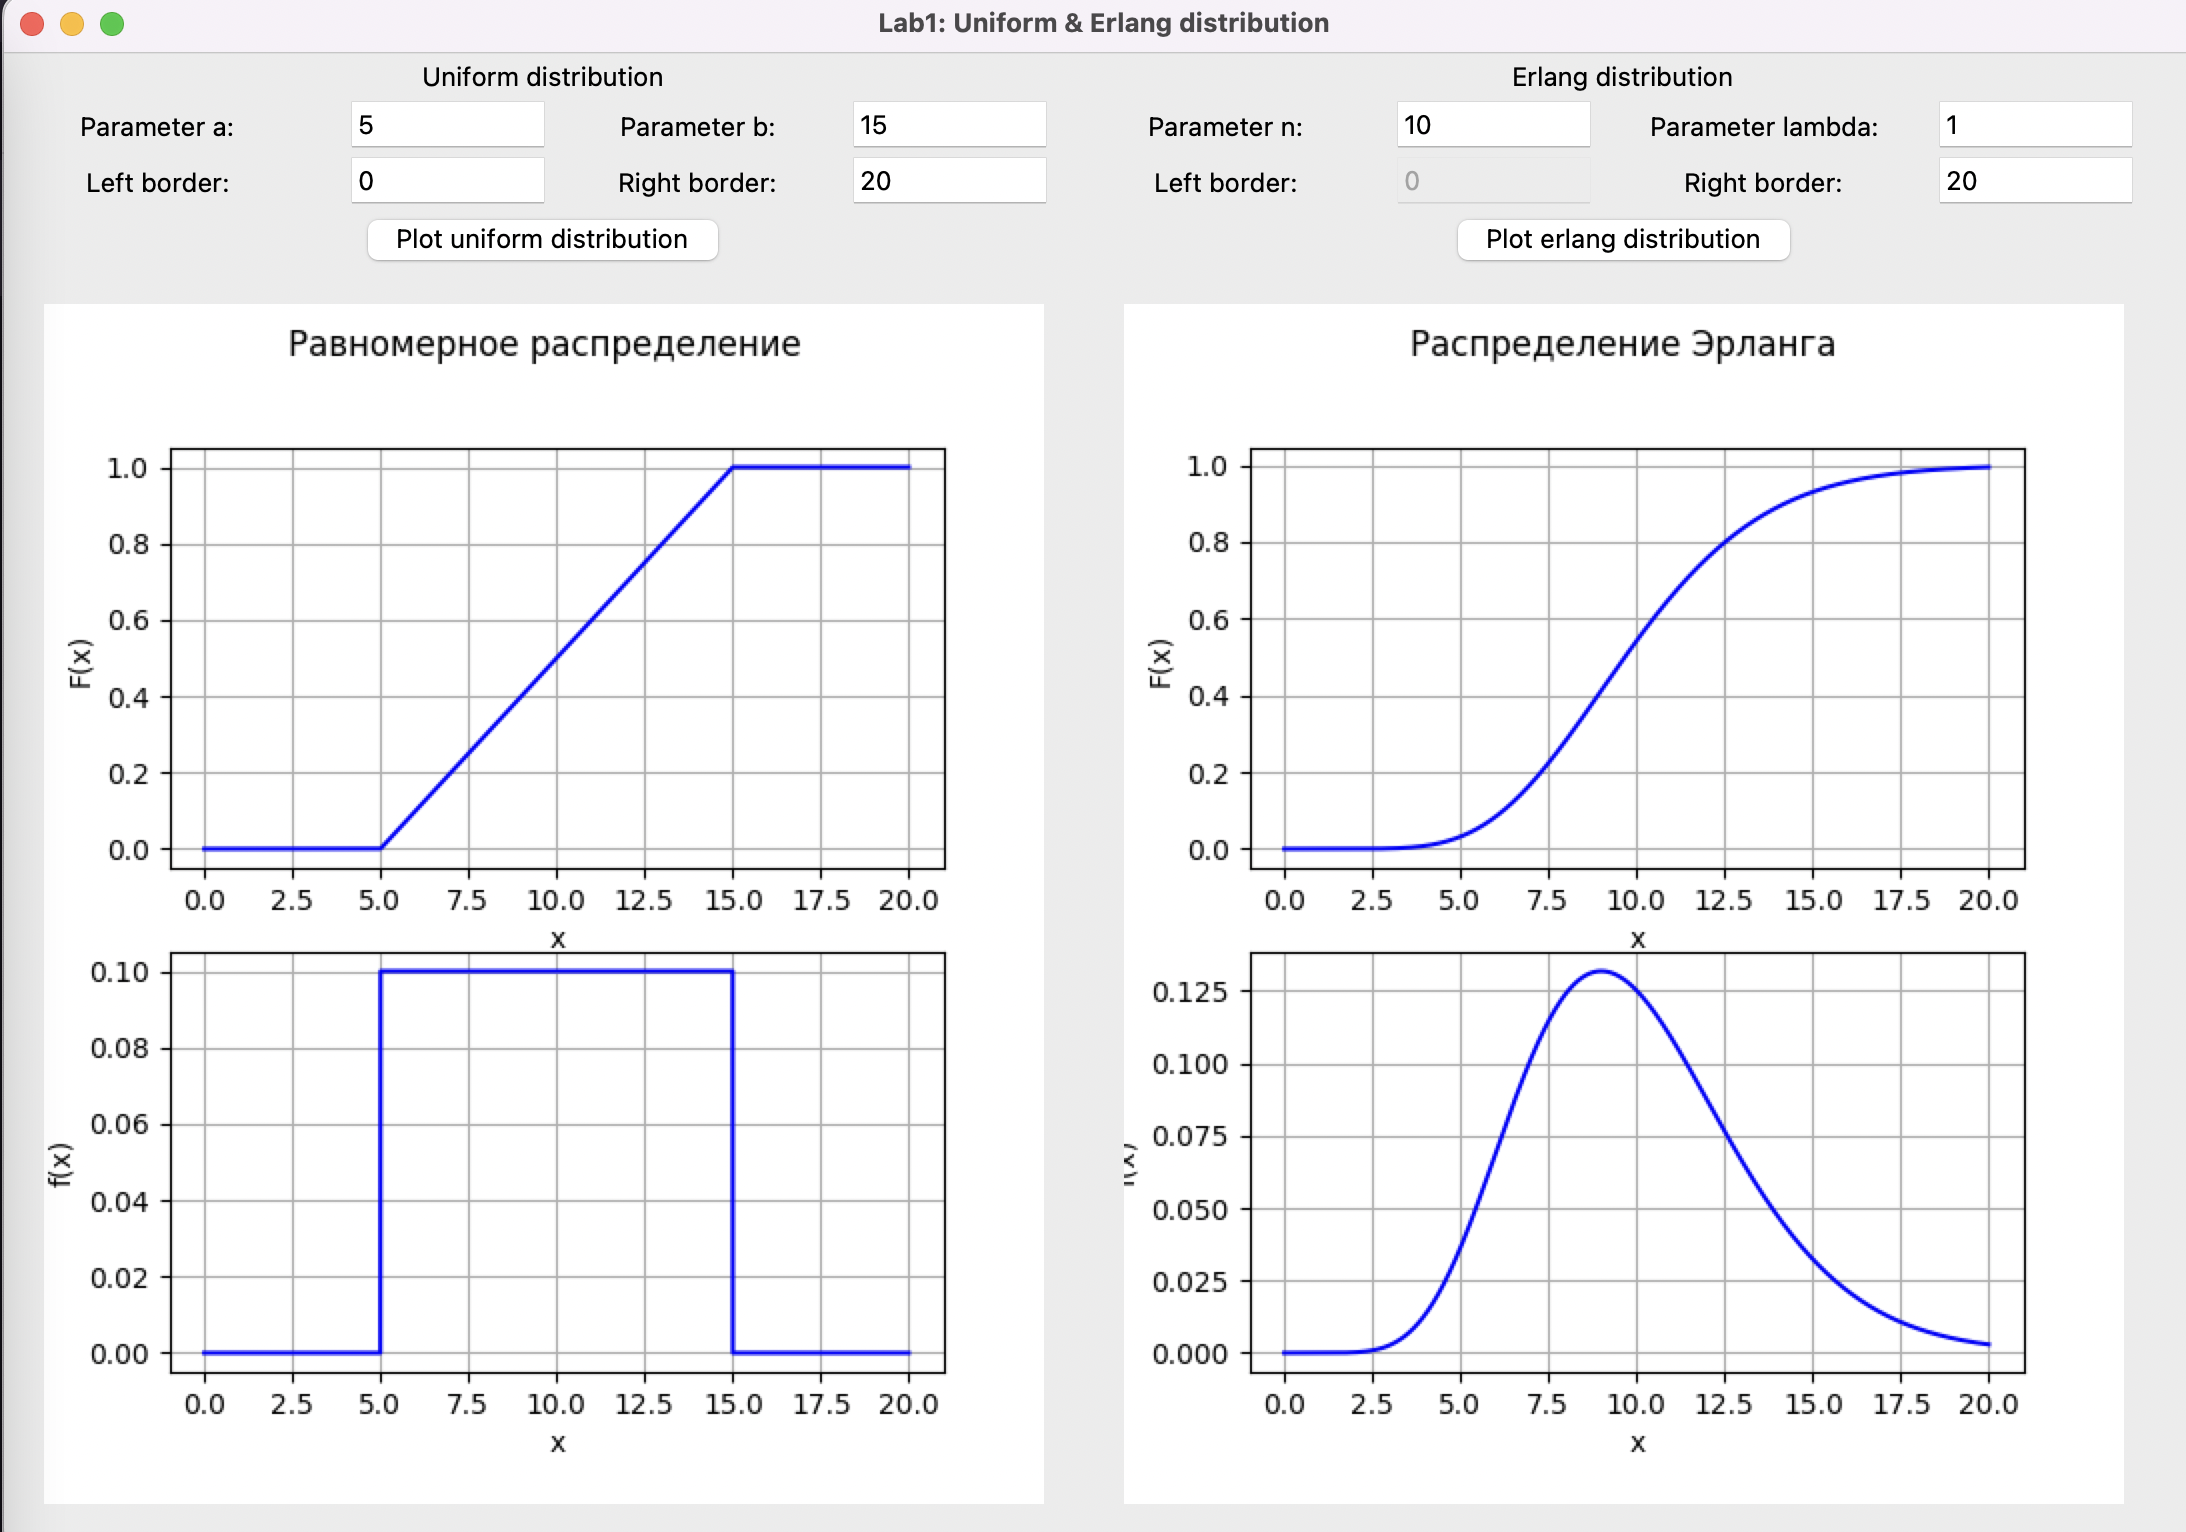
\includegraphics[width=1\textwidth]{inc/pic2.png}
	\caption{Пример работы программы --- 2}
	\label{fig:pic2}	
\end{figure}
\clearpage

На рисунке \ref{fig:pic3} изображен пример работы программы для равномерного распределения с параметрами $a$ = 5, $b$ = 15 на отрезке [0; 20] и для распределения Эрланга с параметрами $n$ = 1, $\lambda$ = 4 на отрезке [0; 20].

\begin{figure}[h!btp]
	\centering
	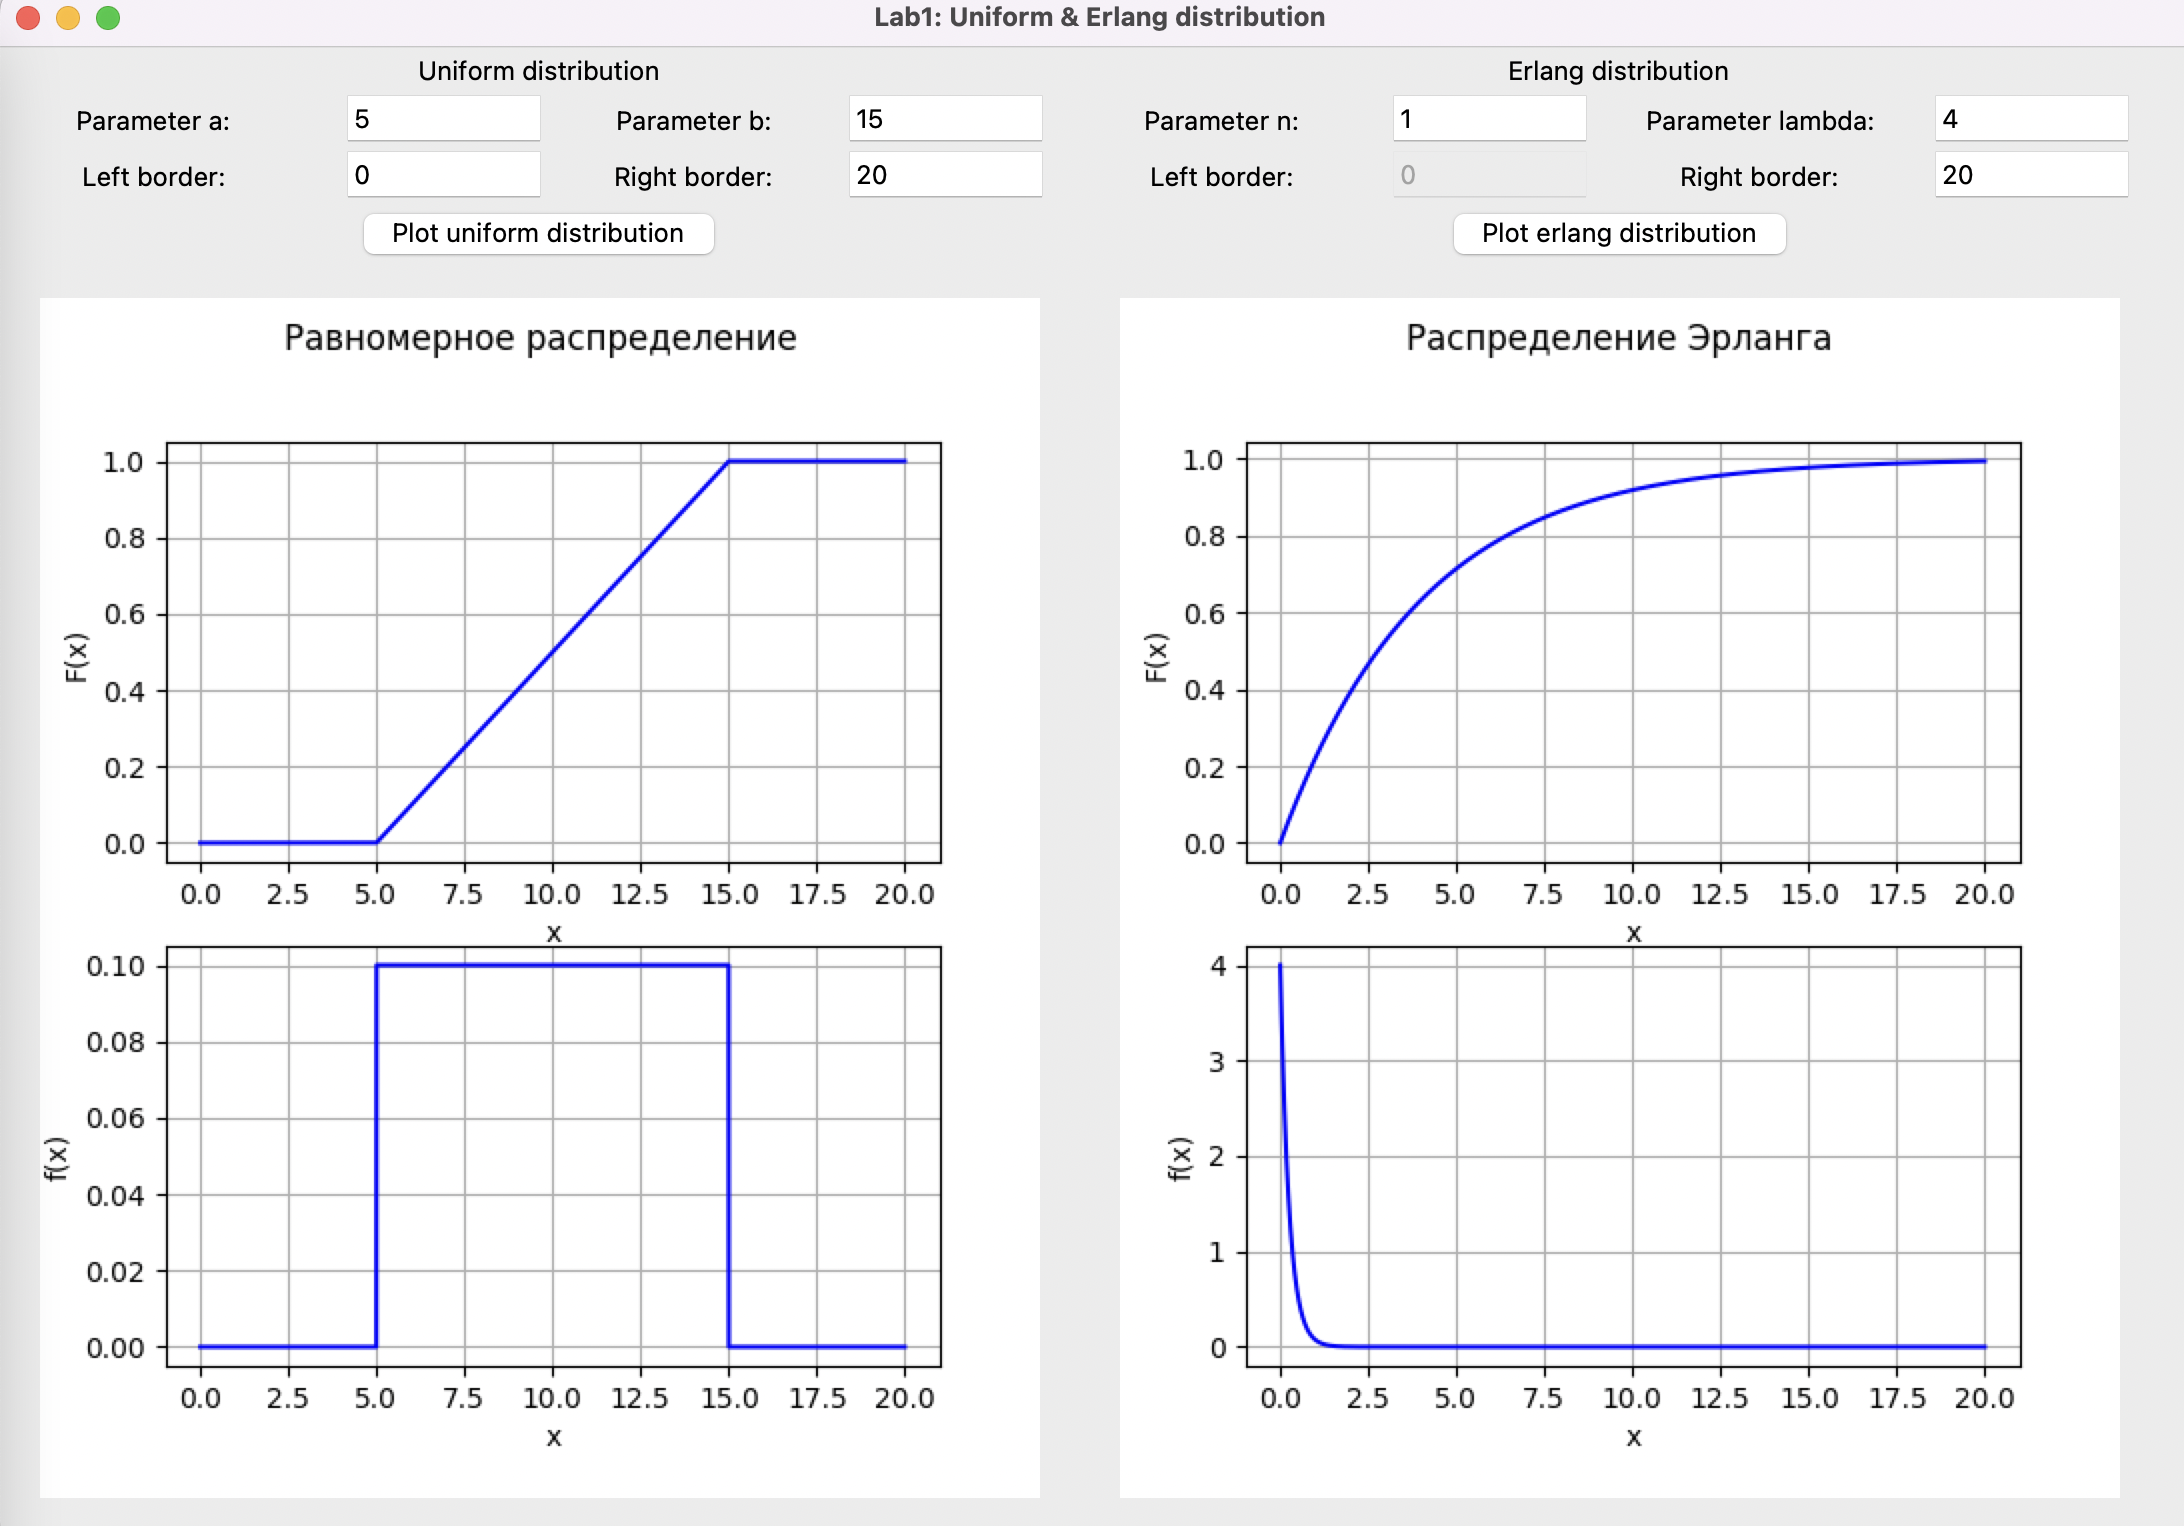
\includegraphics[width=1\textwidth]{inc/pic3.png}
	\caption{Пример работы программы --- 3}
	\label{fig:pic3}	
\end{figure}

\bibliographystyle{utf8gost705u}  % стилевой файл для оформления по ГОСТу
\bibliography{51-biblio}          % имя библиографической базы (bib-файла)
	
\end{document}
